\documentclass[journal]{IEEEtran}

\renewcommand{\baselinestretch}{1.0} % Change to 1.65 for double spacing

\usepackage{amsmath,amsfonts,amssymb}
\usepackage{graphicx}
\usepackage[colorlinks=true, allcolors=blue]{hyperref}


\usepackage{color}
\usepackage[latin9]{inputenc}
\usepackage{mathrsfs,amsmath}
\usepackage{graphicx}%
\usepackage{float}
\usepackage{amsfonts}%
\usepackage{amssymb}
\usepackage{braket}
\usepackage{bm}
%necessary for outline section of the article 
%\usepackage{outline}

\newcommand{\mb}[1]{\bm{#1}}
\usepackage[T1]{fontenc}
\def\Nabla{\bm{\nabla}}
\def\bm{\mathbf}
\def\curl{\Nabla\times}
\def\div{\Nabla\cdot}
\def\lap{\Delta}
\def\vlap{\Delta}
\def\x{\hat{e}_{x}}
\def\y{\hat{e}_{y}}
\def\z{\hat{e}_{z}}
\def\p{\partial}
\def\h{\hat}
\def\tw{\tilde{\omega}}
\def\gm{\gamma}
\def\om{\omega}
\def\OM{\Omega}
\def\GM{\Gamma}
\def\dw{\delta\omega}
\def\dth{\Delta\theta}
\def\dk{\delta k}
\def\Hdth{\frac{\dth}{2}} %half Delta Theta
\DeclareMathOperator{\Tr}{Tr}


\title{Analysis of operating regimes of terahertz quantum cascade laser frequency combs}
\author{\IEEEauthorblockN{Petar Tzenov\IEEEauthorrefmark{1},
		David Burghoff\IEEEauthorrefmark{2},
		Qing Hu\IEEEauthorrefmark{2}, 
		Christian Jirauschek\IEEEauthorrefmark{1}}
	
	\IEEEauthorblockA{\IEEEauthorrefmark{1}Institute for Nanoelectronics, Technical University of Munich, D-80333 Munich, Germany}
	
	\IEEEauthorblockA{\IEEEauthorrefmark{2}Department of Electrical Engineering and Computer Science, Research Laboratory of Electronics, Massachusetts Institute of Technology, Cambridge, Massachusetts 02139, USA}
	\thanks{Corresponding author: P. Tzenov (email: petar.tzenov@tum.de ).}}



\IEEEtitleabstractindextext

\begin{document} 
	\maketitle
	
	
	
\begin{abstract}
In recent years, quantum cascade lasers (QCLs) have shown tremendous potential for the generation of frequency combs in the mid-infrared and terahertz (THz) spectra. The community has experienced success both in the theoretical understanding and experimental realization of QCL devices, capable of generating stable and broadband frequency combs. Specifically, it has been pointed out that four wave mixing (FWM) is the main comb formation process and group velocity dispersion (GVD) is the main comb degradation such. As a consequence, special dispersion compensation mechanisms have been employed, in order to suppress the latter and simultaneously enhance the former processes. Here, we perform detailed computational analysis of four wave mixing, group velocity dispersion and spatial hole burning, all known to play a role in QCLs, and show that SHB has also a considerable impact on whether the device will operate as a comb or not. We thus conclude that for a successful implementation of a quantum cascade laser frequency comb, one would need to seriously address this effect as well. 
\end{abstract}
	
\section{Introduction}
\label{sec:introduction}
The quantum cascade laser frequency comb is an emerging technology with a wide range of applications and most prominently in spectroscopy \cite{schliesser2012mid}. The need for an on-chip direct comb source in the mid- and far-infrared portions of the electromagnetic spectrum has been the main motivation driving the research on this technology. Experimental realizations of combs, first in the midIR \cite{hugi2012mid} and later in the THz \cite{burghoff2014terahertz}, have set the stage for a fruitful discussion on the topic, resulting both in extension of the bandwidth of a THz comb to an octave \cite{rosch2015octave} and also to a series of successful proof-of-concept spectroscopic experiments. Interestingly, it has been also shown \cite{yang2016terahertz} that even given a noisy comb source, one can still perform credible spectroscopic measurements by computationally post-processing the experimental data \cite{Burghoff1601227}.

The generation of a frequency comb by a quantum cascade laser faces some immediate challenges still to be overcome. Specifically, in the THz one of the biggest problems remains the realisation of a room-temperature operating device, or at least one that can be in-expensively cooled while in-use. Unfortunately, due to possibly limitations \cite{albo2015investigating} on state of the art THz QCL designs, the research efforts in this direction have generally stalled, with the current record-holding maximum operating temperature fixed at $approx$ 200 K, remaining unbroken since 2012 \cite{fathololoumi2012terahertz}. Recent work \cite{albo2017temperature}, however, has indicated that if one wants to push this limit higher, serious QCL design re-considerations would need to be implemented.

Temperature performance aside, the general mechanisms contributing to the comb formation and destabilization have been well understood, but due to the complex laser dynamics involved, there still lacks a concrete "recipe" for the making of the perfect QCL frequency comb. Ideally this device should be of very large bandwidth, emit a coherent multimode spectrum with uniform power distribution and also maintain the comb performance over a large dynamic range. Coming up with such a design requires
 quantitatively accurate theoretical models, which depend on as little empirical fitting parameters as possible.

Several recent theoretical treatments \cite{khurgin2014coherent,villares2015quantum}, based on a modal expansion of the electric field and perturbative solution of the density matrix equations, have attempted to fill this gap. However, those approaches nevertheless have some limitations as they do not include the spatial dependence of the modes, assume equidistant mode-spacing, and capture spatial hole burning (SHB) in a somewhat artificial way. As a contrast, in our recent work \cite{petz2016} we have shown that a full time-domain simulation approach, based on a more general set of equations, can represent reality more accurately and still be susceptible to robust analysis.

Broadly speaking, mathematical models of a certain physical system can be simplistic enough as to provide us with analytical solutions and thus intuitive physical insights, or general enough as to be closer to reality but less susceptible to analytical treatment. Therefore our work is based in the latter part of this dichotomy, as we combine accurate numerical schemes with efficient computer implementation to perform simulations of terahertz quantum cascade lasers with high fidelity.

This work can be considered as an extension of our publication in Ref. \cite{petz2016}, as we perform more careful study of the comb formation and comb degradation mechanisms in a typical resonant phonon THz QCL. A major assertion, and probably the main take-home lesson from our research, is our observation indicating that spatial hole burning can play a very large role in the comb degradation process. Our data clearly shows that SHB induces chaotic variation in the phase and amplitude of each lasing mode, resulting in non-comb regime of operation. We further show that upon suppressing of SHB, one can recover the comb character of the laser.  

This paper is organized as follows: in Sec.\ref{sec:theory} we give an overview of the model, introduced in detail in Ref. \cite{petz2016}. In Sec. \ref{sec:proliferation}, we perform a series of what we will call "computational experiments" in order to identify the main mode proliferation mechanism in the device. Section \ref{sec:combdegradation} is dedicated on the analysis of the main comb-degradation effects and lastly Sec. \ref{sec:time-evo} presents results from long time-simulations of free-running, self-starting THz QCLs, demonstrating sufficient conditions for the laser to operate in a comb and non-comb regime. Further, in the same section we show the dramatic effect of spatial hole burning on the comb coherence. In that sense SHB is considered both as a mode proliferation and as a comb-degradation process.

\section{Model}
\label{sec:theory}
Typical resonant phonon THz quantum cascade lasers employ resonant tunneling for effective electron injection into the upper laser level and LO-phonon emission process for rapid depletion of the lower laser state. Due to the ultrafast dynamics of the latter effect, these lasers are known to have very short gain recovery time and spectral bandwidth \cite{wang2015generating}, making them perfect candidates for frequency comb generation. 

Traditional modelling of such devices, depending on the level of complexity, can be divided into four categories: rate equations, Maxwell-Bloch equations (density matrix approach), stochastic Monte-Carlo simulation techniques and fully coherent non-equilibrium Green's function simulations \cite{jirauschek2014modeling} [a good citation for the four approaches?]. A good trade-off between computational efficacy and proximity to the physical reality is provided by the semi-classical Maxwell-Bloch equations, while the rate equations lack the necessary accuracy, and the Monte-Carlo and non-equilibrium Green's function approaches are too computationally demanding for fast prototyping.

Therefore we model the time-evolution of resonant phonon THz QCLs via the Maxwell-Bloch equations. In our previous contribution in Ref. \cite{petz2016} we extended the standard two level Bloch equations to a three level density matrix equations, by including the resonant tunneling coupling between the injector and the upper laser level. We then employed the standard rotating wave and the slowly varying envelope approximations to derive a system of coupled partial and ordinary differential equations modelling the laser under investigation. Similar work had been previously published \cite{callebaut2005importance,kumar2009coherence,dupont2010simplified}, however the authors had focused only on the steady state behaviour and thus neglected transient effects, such as multimode instabilities \cite{wang2007coherent} and temporal hole burning \cite{burghoff2015evaluating}, which have been shown to have immense impact on the laser behaviour. 

Following the reasoning in Ref. \cite{callebaut2005importance}, we consider the resonant tunneling transition between the injector and upper laser levels within the tight-binding approximation \cite{bastard1990wave}.  This allows us to treat the optical and tunneling couplings fully coherently via a density matrix approach, whereas all other scattering mechanisms, e.g. LO phonon, electron-electron, impurity and interface roughness scattering etc., phenomenologically as rate equations. \cite{kumar2009coherence}. 

Considering only the injector state, $\ket{1'}$, and the upper and lower laser levels, i.e. $\ket{3}$ and $\ket{2}$, respectively, the tight-binding Hamiltonian of this system can be written in the rotating wave approximation (RWA) \cite{boyd2003nonlinear} as
\begin{align}
\label{eq:hamiltonian-operatorform}
\h{H}^{\text{RWA}} &= \hbar(\epsilon + \Delta) \h\sigma_{1',1'} +\hbar\Delta\h\sigma_{3,3}  \nonumber \\ &+ (\hbar\Omega_{1'3}\h\sigma_{1',3} +\frac{q_0z_{32}}{2}f \h\sigma_{3,2}+H.c.).
\end{align}
In Eq. (\ref{eq:hamiltonian-operatorform}) we have made the usual ansatz decomposing the electric field $E_z(x,t) = \Re\{f(x,t) e^{i(k_0x-\omega_0t)}\}$ into the product of an envelope function $f(x,t)$ and a carrier wave with central angular frequency $\omega_0$ and wave number $k_0 = n\omega_0/c$. We have implicitly taken that the semiconductor growth direction of the QCL is along the z-axis and thus $E_z$ is the only component of the field coupling to the atomic system. Further, we have denoted with $n$ the background refractive index, with $c$ the velocity of light in vacuum and $z_{32} = \bra{3}\h{z}\ket{2} $ the dipole matrix element between states $\ket{3}$ and $\ket{2}$, where $\h{z}$ is the z-component of the position operator. Also $\hbar\Omega_{1'3}$ denotes the tunneling coupling energy, $\Delta = \omega_{32} -\omega_0$ is the detuning of the electric field from $3\leftrightarrow 2$ resonance and we have set the energy of the lower level to zero, i.e. $E_2 = 0$. Finally, $\h \sigma_{i,j}$ denotes the atomic projection operators and "$H.c$" the Hermitian conjugate.

The state of the three level system at any point in time is captured by the density matrix operator $\h{\rho}^{\text{RWA}}$, which is also taken in the RWA. The time evolution of this quantity is given by
	\begin{equation}
	\label{eq:vonNeumann}
	\frac{d \h{\rho}^{\text{RWA}}}{dt} = -\frac{i}{\hbar}[\h{H}^{\text{RWA}};\h{\rho}^{\text{RWA}}] + \left.\frac{d\h{\rho}^{\text{RWA}}}{dt}\right|_{\text{coll}},
	\end{equation}
	where $[\cdot;\cdot]$ is the usual quantum mechanical commutator and the last term denotes the phenomenologically included "collision terms" modelling the interaction of this system with the environment.

	In order to complete the description of the system, we simulate the time evolution of the forward and backward travelling components of the field envelope with the aid of a pair of propagation equations, and we also extend Eq. (\ref{eq:hamiltonian-operatorform}) accordingly,  to include  spatial hole burning (SHB) \cite{gordon2008multimode}, as well as the effect of additional laser levels from a single period of the active region. Since the resulting system of equations has been published elsewhere \cite{petz2016}, we omit further details on the technicalities, and instead focus our attention on the possible applications of our model for QCL device characterization. 
	
	\section{Mode proliferation mechanisms}
	\label{sec:proliferation}
	
	Both theoretical \cite{khurgin2014coherent} and experimental \cite{friedli2013four} investigations have confirmed that four wave mixing (FWM), induced by the large third order non-linearity $\chi^{(3)}$, acts as the main comb-formation mechanism in free running mid- and far-infrared QCL devices.
	
	For example, a series of pump-probe experiments were performed in Ref.~\cite{friedli2013four}, where a mid-IR QC amplifier was pumped with two single mode lasers, emitting a pair of frequencies, $f_1$ and $f_2$ (with $f_1 > f_2$), lying well under the gain spectrum of the device. Outcoupled light was consecutively recorded and subsequent spectral analysis revealed the clear footprints of degenerate four wave mixing, i.e. the generation of a pair of conjugate modes at the Stokes and anti-Stokes frequencies of  $f_s = 2f_2 -f_1 $ and $f_a = 2f_1 - f_2 $, respectively. Combined with the inherently broadband gain of QCLs, this effect could support the generation of more sidebands in a cascaded manner, ideally spanning the full bandwidth of the laser. Since FWM is an energy conserving process, in this way it ought to lead to an equidistant multimode spectrum and thus a frequency comb.
	
	Unfortunately, this not always occurs due to the competition of FWM with various comb-degradation mechanisms such as group velocity dispersion (GVD) and multimode instabilities such as the Risken-Nummedal-Graham-Haken (RNGH) instability \cite{risken1968self,graham1968quantum}, argued to be with a lower threshold in QC lasers due to spatial hole burning (SHB) \cite{gordon2008multimode}. From these the former, i.e. GVD, has been shown \cite{burghoff2015evaluating,villares2016dispersion} to play a major role in blocking the formation of a nice equidistantly-spaced spectrum. That is why state of the art QCL frequency combs usually employ sophisticated dispersion compensating mechanisms (DCMs), either based on a chirped corrugation structures embedded into the laser cavity \cite{burghoff2014terahertz} or GTI-mirrors positioned behind one of the facets of the laser \cite{villares2016dispersion}. Both techniques have shown to be very successful in eliminating the dispersion, leading to comb formation, however there is still lack of clear understanding as to why lasers operating at negative GVD are easier to phase-lock \cite{villares2016dispersion} or why are the DCMs effective only within a narrow range from the overall operating regime~\cite{burghoff2014terahertz}.
	
	\begin{figure}[h!]
		\centering
		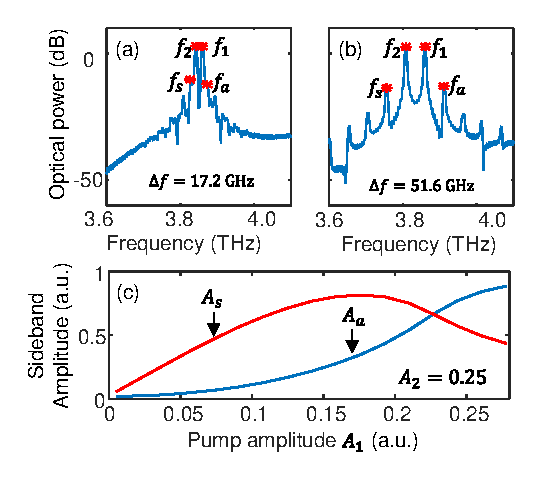
\includegraphics[width=0.40\textwidth]{IMGS/FWM_PROOF}
		\caption{(a) Optical spectrum obtained from THz-TDs simulations with two seed modes $f_1$ and $f_2$, separated by $\Delta f = 17.2$ GHz. The sidebands, detected at $f_s$ and $f_a$, with corresponding amplitudes $A_s$ and $A_a$, denote the FWM-generated Stokes and anti-Stokes waves. (b) same as (a) however the pump modes are separated by $\Delta f = 51.6$ GHz. (c) Dependence of the amplitudes of the sidebands, when the strength of the first pump at $f_1$ is varied, while $A_2$ is kept constant.  }	\label{fig:FWM_proof}
	\end{figure}
	
	Within our model, we can investigate the effect of different parameters on the efficacy of FWM by essentially emulating laboratory experiments similar to those in Ref. \cite{friedli2013four}. Figures \ref{fig:FWM_proof}(a) and \ref{fig:FWM_proof}(b) show data from two such computations, when we simulated a laser, seeded through the left facet with two equally strong pump modes with frequencies $f_1$ and $f_2$, when we varied the mode spacing  $\Delta f = f_1 - f_2$. In both cases, the simulations were based on the THz QCL from Ref.~\cite{burghoff2014terahertz}, biased at 11 kV/cm. All scattering rates and other relevant active region parameters were calculated with the aid of our Schroedinger-Possion and ensemble Monte Carlo codes~\cite{jirauschek2014modeling} and their values are not considerably different from the data published in Ref.~\cite{petz2016}. Importantly, here we set the left and right amplitude reflectivities to only 5\%, in order to eliminate spatial hole burning from the simulation and thus isolate FWM as the only mode proliferation mechanism.
	
	The logarithmic optical power spectrum clearly shows the emergence of signals at the Stokes and anti-Stokes frequencies only after 10 round trips of the light inside a linear cavity of length $L = 2.5$ mm.  Based on the formalism in \cite{sutherland2003handbook}, we know that the amplitudes of the generated sidebands at $f_a$ and $f_s$ will experience the following dependence on the pump amplitudes, i.e. $A_{1}$ and $A_{2}$, and the nonlinear susceptibility $\chi^{(3)}$:
	\begin{align}
	A_{a} &\propto \chi^{(3)}(f_1,-f_2,f_1;-f_a) A_{1}^2 A_{2}, \nonumber \\
	A_{s} &\propto \chi^{(3)}(-f_1,f_2,f_2;-f_s) A_{1}  A_{2}^2. \label{eq:susceptibility}
	\end{align}
	
	Figure \ref{fig:FWM_proof}(c) shows namely this dependence when the strength of the first pump at $f_1$ is varied, whereas all other parameters are kept fixed. We see that, in the weak pumping regime, $A_{s}$ demonstrates linear dependence on $A_{1}$, whereas $A_{a}$~-quadratic. Further, we also observe saturation effects and, more interestingly, the previously reported in experiment~\cite{friedli2013four} threshold behaviour of $A_{a}$, emerging only after $A_{1}$ is large enough as compared to $A_2$.
	
	Even though our approach lacks the robustness of a direct mathematical proof, we believe that these results unequivocally confirm that it is indeed four wave mixing which is observed, and not other multi-mode generation effect. In principle Eq.~(\ref{eq:susceptibility}) could also be used to computationally extract the spectral shape of the third order susceptibility of the modelled QCL, but due to insufficient experimental data for comparison we deter this to possibly a later publication. 
	
	%\begin{figure}[h!]
	%	\centering
	%	\includegraphics[width=0.40\textwidth]{IMGS/shb_graph.eps}
	%	\caption{Graphical representation of SHB. The upper image depicts the formation of standing waves in the intensity due to counter-propagating fields. The second row illustrates the corresponding inversion grating. The unequal saturation along the cavity length could lead to the emission of "secondary" waves with anti-nodes located at the saturation minima. Adapted from \cite{siegman1986lasers}.}	\label{fig:shb_graph}
	%\end{figure}
	
	An additional mode proliferation mechanism, highly relevant for quantum cascade lasers, is spatial hole burning. This effect arises due to interference effects of counter propagating waves in lasers with Fabry-Perot type cavities, and it has been shown \cite{wang2007coherent,gordon2008multimode,gkortsas2010dynamics} to induce multimode instabilities and also hamper active mode locking of QCL devices. The principle, under which SHB leads to multimode lasing, is straightforward to understand \cite{siegman1986lasers}. The superposition of two cavity modes  $E_j(x,t) = \Re\{A_j(x)\exp[i(k_jx-\omega_jt)]\}$, with $j =\{1,2\}$ denoting the mode index, would produce an intensity interference pattern 
	\begin{equation}
	\label{eq:interference-effect}
	I(x,t) = I_1+I_2+2\sqrt{I_1I_2}\cos((\omega_2-\omega_1)t-(k_2-k_1)x+\delta\phi),
	\end{equation}
	where $I_j \propto |A_j|^2$, denotes the intensity of each mode, $\omega_j$ and $k_j$ the corresponding angular frequencies and wave numbers, respectively, and $\delta\phi = \phi_2-\phi_1$ the phase difference. Now, assuming that both waves have the same frequency, i.e. $\omega_1 =\omega_2$, but propagate in opposite directions, $k_1 = -k_2$, we immediately see that the intracavity intensity will form a standing wave pattern with wavelength equal to half the wavelength of the original mode. Due to saturation effects the population inversion will experience spatial dependence of the form 
	\begin{equation}
	\frac{\Delta N(x)}{N} = \frac{1}{1+I(x)/I_{sat}}, 
	\end{equation}
	where $N$ is the average carrier density $\Delta N(x)$, is the spatial dependent inversion and $I_{sat}$ is the saturation intensity. In such a scenario secondary modes, with anti-nodes located at positions where the saturation due to the main, i.e. the primary mode, is weak, could experience a net gain and thus begin to lase. 
	%This process is schematically illustrated in Fig.~\ref{fig:shb_graph}. 
	
	It has been also argued that spatial hole burning might destabilize the comb emission as it could lead to strong amplitude and phase fluctuations. The mechanism with which this occurs is namely the RNGH instability, which has been shown to have lower threshold in QCLs, when SHB is taken into account \cite{gordon2008multimode}. This means that whenever the pump current is above this instability threshold, spatial hole burning can severely alter the laser dynamics and ultimately act as a comb-degradation mechanism.
	
	\section{Comb degradation mechanisms}
	\label{sec:combdegradation}
	
	\begin{figure*}[tb]
		\centering
		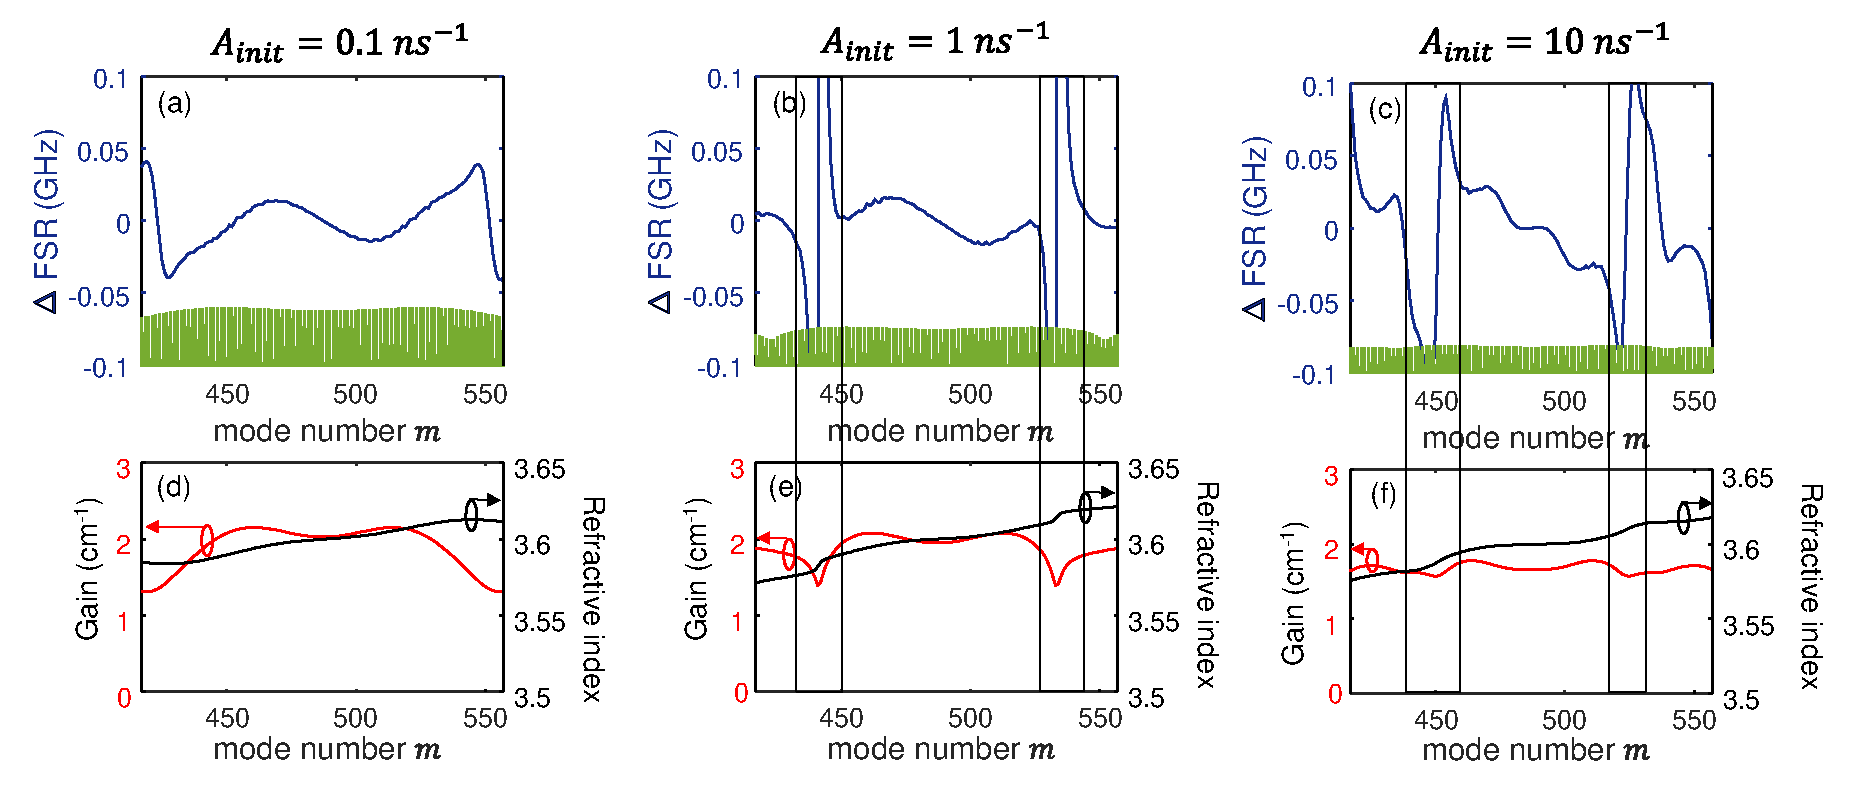
\includegraphics[width=0.85\textwidth]{IMGS/FSR_variation}
		\caption{Results from simulations of a numerical pump-probe experiment, performed with our model in Ref. \cite{petz2016}. (a), (b) and (c) display the variation of the free spectral range, as a function of the mode index $m$, for values of the pump  pulse amplitude, normalized to the Rabi-frequency, at 0.1 ns$^{-1}$, 1 ns$^{-1}$ and 10 ns$^{-1}$, respectively. For illustrative purposes we also plot the cavity modes (green lines), calculated via $f_m = m\times c/2Ln'(f_m)$, with amplitudes weighted by the normalized gain. (d), (e) and (f) Spectral gain (left y-axis) and the real part of the refractive index (right y-axis) as a function of the mode index $m$ and the pump pulse amplitude. All simulations were performed at value of the applied bias of 11 kV/cm, where the upper-lower laser level transition frequency was calculated at $f_0 = 4.05$ THz. The refractive index at $f_0$ was set to $n=3.6$ and the simulated cavity length was chosen as $L=5$ mm, giving a free spectral range $FSR(f_0) = 8.3$ GHz and a corresponding central mode index $m_0 = 487$.}	\label{fig:dispersion}
	\end{figure*}
	
	It is known that chromatic dispersion in a device, i.e. frequency dependence of the refractive index, effects the equidistance of the Fabry-Perot modes, and thus hampers the formation of a comb. Direct estimation of the GVD of a device is difficult, as it has a strong dependence on the system parameters, waveguide design, as well as the power spectral density of the lasing modes (due to self- and cross- phase modulation effects) \cite{villares2016dispersion}. This also makes the theoretical treatment very challenging and therefore impedes the computer aided design of QCL frequency combs.
	
	Again, we find that the Maxwell-Bloch equation provide us with a  suitable framework for the rigorous treatment of dispersion, as the density matrix equations intrinsically capture polarization effects, and thus dispersion due to optical gain. The model can be extended by the phenomenological inclusion of different dispersive components, e.g. waveguide or bulk dispersion, via complementary ordinary differential equations, modeling this additional material response in the time domain \cite{taflove2000computational}.
	
	We restrict ourselves to modelling only dispersion due to optical resonances, i.e. gain dispersion, and in the following we perform several computational experiments to characterise its impact on the equidistance of the cavity modes.
	
	The general idea is to treat the gain medium of length $L$ as a nonlinear filter with some unknown transfer function $H(\omega)$. If were able to extract the magnitude and frequency response of this transfer function, we could use this information to infer the real and imaginary part of the refractive index. This can be done quite easily by simulating the passage of a pulse, with suitably chosen spectral width and amplitude, through the medium, recording the pulse at the output facet of the simulation region, and finally processing the input and output data in frequency domain~\cite{petz2016}. The real power of this method lies in its universality, as it allows us to characterize the time-dependent behaviour of the system under different operating conditions, by simply varying the model parameters.
	
	From basic laser theory~\cite{siegman1986lasers}, we know that a Fabry-Perot cavity of length $L$ will sustain longitudinal modes, determined by the relation $f_m = m \times c/2 L n'(f_m),$ where $m$ is some (large) integer, $f_m$ denotes the $m^{\text{th}}$ mode, $c$ the velocity of light in vacuum and $n'(f_m)$ is the corresponding value of the real part of the refractive index. The spacing at the $m^{\text{th}}$ longitudinal mode is also known as the free spectral range (FSR) and is given by $FSR(m)=f_{m+1}-f_{m}\approx c/2 L n'(f_m)$, which is generally index-dependent.
	
	In free-running QCLs, due to their broadband nature and ultrafast carrier dynamics \cite{khurgin2014coherent}, there will be a strong competition between FWM and dispersion, the outcome of which will determine the free spectral range. This is because, while the former is an energy conserving process and thus tends to homogenize the mode spacing, the latter has a detrimental influence as it results in an FSR depending on frequency. It has been shown \cite{rosch2015octave} that at operation regimes where the different components of dispersion cancel each other out, or when special dispersion compensation mechanisms are employed \cite{burghoff2014terahertz}, four wave mixing can defeat intracavity dispersion, via the injection-locking effect \cite{siegman1986lasers}, resulting in a broad comb spectrum. Generally, however, those comb regimes cover only a fraction of the whole dynamic range of the device and are usually limited to near-threshold operation. In fact, a clear explanation of why FWM looses to GVD   is somehow missing. It has been suggested \cite{villares2016dispersion} that in cases of large dispersion the phase-matching condition for FWM is violated and therefore the process becomes inefficient. 
	%higher values of the injection current the appearance of more modes in the lasing spectra, up to the boundaries of the spectral gain,  increases the deteriorating effect of dispersion due to the larger values of the GVD coefficient at the periphery of the gain curve.
	However, in our previous work \cite{petz2016} we showed via a simple Taylor expansion that, for the type of FWM depicted above, values of the GVD coefficient as high as 2 ps$^2/$mm cannot introduce a sufficiently strong phase-mismatch. We would like to report that we observe another comb-degrading effect, which can be related to spatial hole burning-induced instabilities, and could be also one of the reasons for the breakdown of comb-like operation at high pump currents.  
	
	First, we investigate in detail the frequency dependence of the refractive index, we the aid of the computational trick, outlined in the beginning of this section, when we vary the amplitude of the input pump pulse. In doing so, we can analyze the net effect of different intensity-dependent phenomena, such as gain saturation and also self and cross-phase modulation, onto the system dynamics. 
	
	For these simulations we take the the QCL of Ref. \cite{burghoff2014terahertz}, again by applying our model from Ref. \cite{petz2016}. This time, we set the cavity length to $5$ mm and propagate the pump pulse only once before post processing. Figure \ref{fig:dispersion} illustrates the results from this procedure when we vary the strength of the input pulse. The latter is chosen as an unchirped Gaussian, with intensity full-width at half maximum (FWHM) of $1$ ps,  corresponding to a FWHM bandwith of 440 GHz (from the time-bandwidth product), whereas the amplitude is normalized to the Rabi-frequency of the material. 
	
	As a figure of merit for the effect of chromatic dispersion on the comb-spacing, we calculate the frequency dependent variation of the free spectral range \cite{herr2012universal} via 
	\begin{equation}
	FSR(m) = (f_{m+1}-f_{m}) - (f_{m} - f_{m-1}).
	\end{equation} 
	Figures~\ref{fig:dispersion}(a)-\ref{fig:dispersion}(c) illustrate the dependence of $\Delta FSR$ upon the pump pulse intensity. For completeness, we also plot, Figs.~\ref{fig:dispersion}(d), \ref{fig:dispersion}(e) and \ref{fig:dispersion}(f), the shapes of the calculated spectral gain and the real part of the refractive index. 
	
	The plots in Fig. \ref{fig:dispersion}(a)-\ref{fig:dispersion}(f) show large variations in $\Delta FSR$ upon gain saturation. This is due to the fact that casuality \cite{toll1956} imposes an intimate relationship between the real and imaginary parts of the refractive index, via the Kramers-Kronig relations.  In particular, we see from Figs.~\ref{fig:dispersion}(b)-(c) and \ref{fig:dispersion}(e)-(f), that at places where the saturated spectral gain has a large curvature, due to the dependence $\Delta FSR(m) \propto \partial^2 f_m/\partial m^2 $, this would lead  to strong variation of the free spectral range and thereby very uneven mode spacing. This reveals to us that dispersion control is a highly non-trivial problem, deeply rooted in the laser dynamics ( e.g. the fluctuations in the mode intensities), which might explain the difficulties of designing a dispersion compensation mechanism which can be effective over a broad range of operating conditions. The authors acknowledge the need to further extend the current theoretical model, in order to be able to include more complicated dispersion relations in future simulations. 
	
	As mentioned in the previous section, spatial hole burning is directly related to amplitude and phase instabilities in QCLs due to the effective lowering of the RNGH-threshold, and therefore deserves a more detailed study.  A thorough analytical investigation of SHB was already performed in Ref. \cite{gordon2008multimode} via a linear stability analysis of the Maxwell-Bloch equations. The authors managed to show how, in the presence of spatial hole burning, a two level system with a gain recovery time $T_1$ and a dephasing time $T_2$, will experience parametric gain, with maximum values at frequencies separated from the central frequency by the following distance-squared:
	\begin{equation}
	\Omega_{max}^2 \approx \frac{1}{T_1} \sqrt{\frac{p-1}{3T_1T_2}},
	\end{equation}
	where $p$ is the pump parameter and $p=1$ means that the laser is biased exactly at threshold. When driven high above threshold, many QCLs, candidates for frequency comb emitters, show the predicted by the above formula spectral splitting, confirming the correctness of the analysis~\cite{wang2007coherent}.
	
	Ideally, SHB will not play a significant effect if the pumping is weak, i.e. $p\approx 1$, or the peaks of the parametric gain are well outside the gain full width at half maximum bandwidth, i.e. $\Delta\nu_{FWHM}$. Assuming, for simplicity, that $T_1 \approx T_2$, we could impose the condition 
	\begin{equation}
	T_1 \ll T_1^{max} = \frac{1}{\Delta\nu_{FWHM}}\sqrt{\frac{p-1}{3}},
	\end{equation}
	from where we see that for lasers with extremely fast gain recovery, spatial hole burning could not be expected to play a significant role. How fast should this gain recovery time be? Well, this obviously depends on the strength with which one pumps above threshold, but for value of $p=2$, for example, and a value of $\Delta\nu_{FWHM}\approx 2\pi\times 1$ THz, this yields $T_1^{max}\approx 0.06 $ps, which is unfortunately an order of magnitude too fast to be realistic. 
		\begin{figure*}[tb]
			\centering
			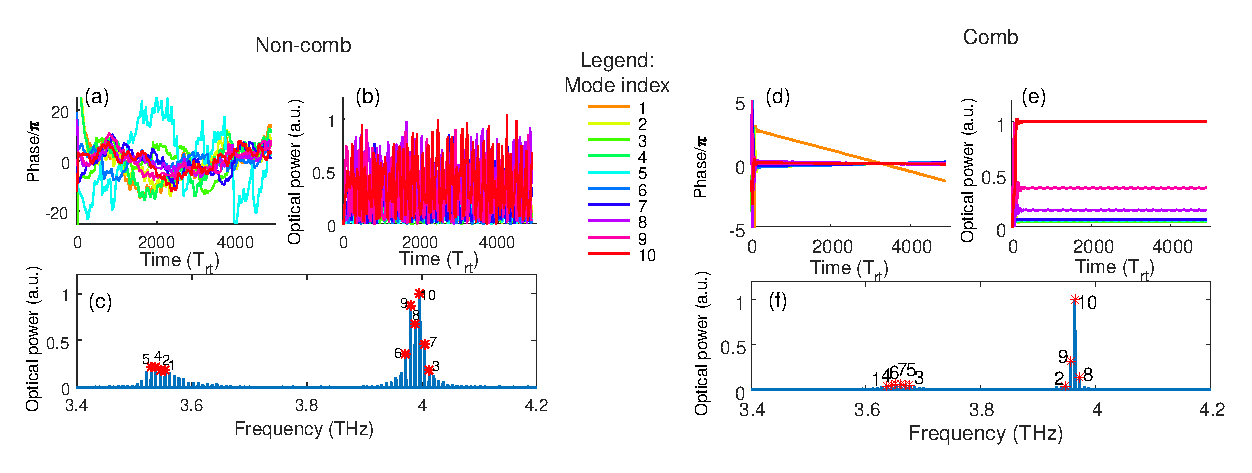
\includegraphics[width=0.8\textwidth]{IMGS/COMB_vs_NOCOMB1}
			\caption{Simulations of non-comb and comb regime of operation of a THz QC laser. These simulations are identical to the ones presented in Ref. \cite{petz2016}. (a) (b) and (c) modal phase, power and overall spectra of a dispersion uncompensated device. (d), (e) and (f) modal phase, power and overall spectra of a dispersion compensated device. The modal phases and powers were obtained via the short-time Fourier transform with a Hanning window function of duration 5 round trips (round tip time is approximately 120 ps) for a total simulation time of 5000 round trips. The phases are presented after filtering out the constant linear time-drift, obtained with least squares estimation. We plot the results for the 10 strongest modes in the corresponding spectra in c) and f), the locations of which are indicated by star-shaped markers.  The colour coding for each modes is presented in the legend (coloured version on-line)}	\label{fig:combnocomb1}
		\end{figure*}
	
	Another method to suppress spatial hole burning is by incorporating the gain medium into a ring cavity instead of a Fabry-Perot one. In Ref. \cite{revin2016active} it has been demonstrated that integrating the active region into an external ring cavity leads to dramatic improvement of the quality of active mode locking and consecutively the emission of short pulses by a mid-IR QCL, known to be infamously hard to mode lock. A more accessible method for reducing SHB is by creating a cavity with asymmetric mirror reflectivities such that the outcoupling is much stronger at, for example, the right facet of the cavity than the left. In such a scenario, the intensity of the right to left propagating component of each mode will be much smaller than the one in the opposite direction, which will lead to suppression of the interference term in Eq. (\ref{eq:interference-effect}) and thus reduction of the depth of the inversion grating. In the next section, we simulate this latter scenario and show how, when SHB is weak, a free running laser could settle in a regime of stable phase- and amplitude-coherent operation and therefore emit a frequency comb.

	\section{Time-evolution of the multimode spectra in QC lasers}
	\label{sec:time-evo}
	
	
	In the following we present results from long-time simulations of our hypothetical THz QC laser for a self-starting, free running configuration under different boundary conditions. Within our analysis, we find that spatial hole burning has a dramatic effect onto the comb performance, one that appears even more relevant than dispersion. To see how SHB affects the dynamics, we need therefore to conduct a more detailed study of the time evolution of the phase and amplitude of each of the lasing modes in the spectrum. 
	
	In order to establish a criterion as to what this time evolution should be in the case of a comb and a non-comb regime of operation, we first we reproduce our previously published results in Ref. \cite{petz2016}. There we performed simulations of the same device, treated above, with and without dispersion compensation, showing that in the former case the laser emitted a comb, whereas in the later - an incoherent multimode spectrum. Here we present a deeper look into our data, where we track the time-evolution of the amlitudes and phases of the top 10 strongest lasing modes in the two cases. 
	
	The results are summarized in Fig. \ref{fig:combnocomb1}. A quick comparison of the different plots reveals a striking difference in the time-domain dynamics of both scenarios. In Figs.~\ref{fig:combnocomb1}(a) and \ref{fig:combnocomb1}(b), demonstrating the non-comb operational regime, we observe chaotic fluctuation of phase and amplitude without any noticeable regularity or tendency for convergence. In fact, it almost seems that all individual modes switch on and off at random time intervals. This is namely a manifestation of multimode phase and amplitude instabilities discovered independently by Risken and Nummedal~\cite{risken1968self} as well as Graham and Haken~\cite{graham1968quantum}. In contrast, whenever the laser operates as a comb, i.e. Figs.~\ref{fig:combnocomb1}(d) and \ref{fig:combnocomb1}(e), after several hundred round trips the lasing modes quickly converge to their steady state values with very little variation what so ever. Thus the modes are lasing constantly and are clearly phase-locked. 
	
	\begin{figure}[h!]
		\centering
		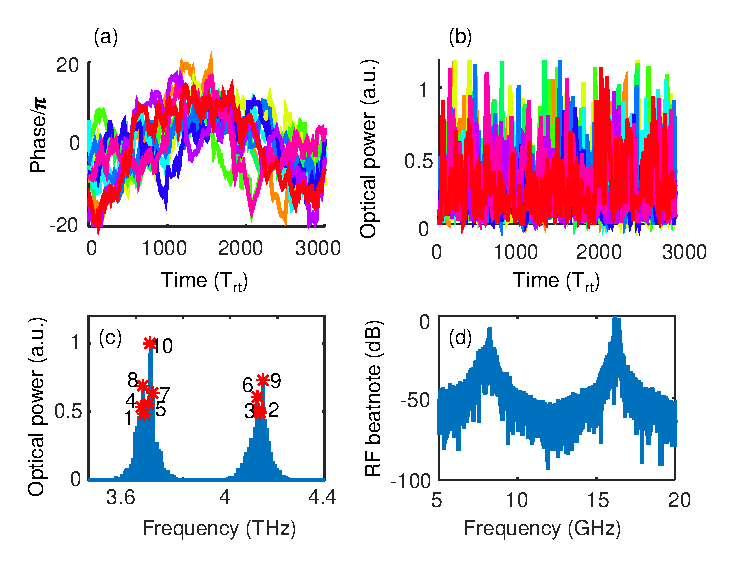
\includegraphics[width=0.45\textwidth]{IMGS/NOCOMB_NODISP}
		\caption{Simulation results of a free-running THz QCL, biased at 11 kV/cm, where both the left and the right facet reflectivities were set at 100\%, in order to support a \emph{strong} spatial hole burning effect. (a) and (b) illustrate the modal phase and power of the top ten strongest lasing modes in the spectrum. (c) Optical power spectrum (normalized) and (d) radio-frequency (RF) beatnote of the simulated device. The modal characteristics, i.e. (a) and (b), were extracted using the short-time Fourier transform with a Hanning window of 5 round trips over a total simulation time of 3000 round trips. The colour coding is identical to Fig. \ref{fig:combnocomb1} (colour on-line).}	\label{fig:NOCOMB_NODISP}
	\end{figure}
	
	Now, we investigate whether SHB has any impact on the laser spectrum. First we simulate the device under study, biased at 11 kV/cm, in a free-running regime of operation when both outcoupling mirror reflectivities were set to 100\%. Since equal facet reflectivities strongly favour the formation of standing waves and thus the onset of SHB. 
	
	Unsurprisingly, our simulation results reveal a similar behaviour to the one in Figs.~\ref{fig:combnocomb1}(a)-\ref{fig:combnocomb1}(c), with chaotic variation of the spectral modes in Figs.~\ref{fig:NOCOMB_NODISP}(a)-\ref{fig:NOCOMB_NODISP}(b) and a multi-beatnote signal around $f_{rt} = 8.3$ GHz, Figs.~\ref{fig:NOCOMB_NODISP}(d). Thus, quite expectedly, when there is no dispersion compensation and spatial hole burning is strong, the laser fails to produce a comb.
	
	\begin{figure}[h!]
		\centering
		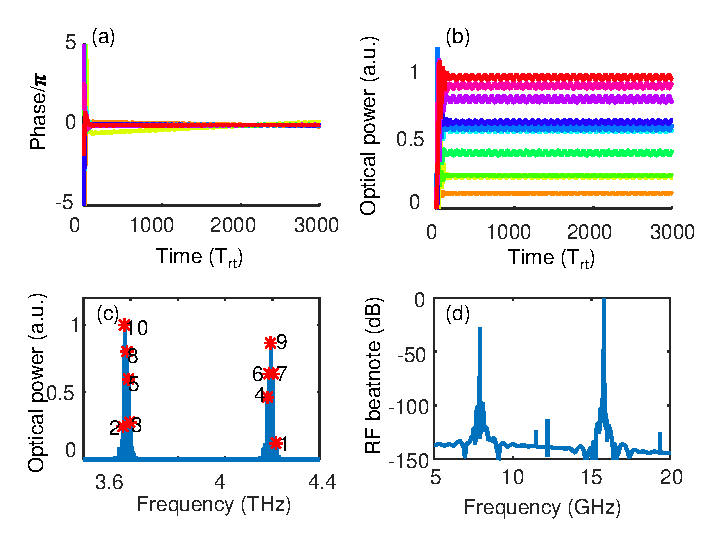
\includegraphics[width=0.45\textwidth]{IMGS/COMB_NODISP}
		\caption{Simulation results for the same configuration as in Fig. 
			\ref{fig:NOCOMB_NODISP}, with the difference that the right reflectivity coefficient was set to 5\%, whereas the left was maintained at 100\%, in order to support a \emph{weak} spatial hole burning effect. (a) and (b) depict the modal phase and power of the top 10 strongest modes, visible in the optical spectrum in (c). (c) Optical spectrum produced by the simulation with the top 10 modes indicated by red star-shape markers and corresponding mode index. (d) RF beatnote, calculated from the simulation.}	\label{fig:COMB_NODISP}
	\end{figure}
	
	Next, we performed simulations with asymmetrically chosen outcoupling losses, where the left reflection coefficient was maintained at 100\% and the right one was set to 5\%. As discussed in Section \ref{sec:combdegradation}, this strengthens the unidirectionality of the emission and thus suppresses SHB. Notice that no dispersion compensation has been employed here, in contrast to the simulation results in Figs. \ref{fig:combnocomb1}(d)-\ref{fig:combnocomb1}(f). The plots in Figs. \ref{fig:COMB_NODISP}(a)-\ref{fig:COMB_NODISP}(d) show that by only eliminating spatial hole burning we can recover the comb-like stable behavior. Two things in our data are obvious and need to be considered more carefully. 
	
	First, comparing the spectra of Fig.~\ref{fig:NOCOMB_NODISP}(c) and Fig.~\ref{fig:COMB_NODISP}, we observe a decrease in the number of lasing modes. This comes naturally, since clamping of the gain around it's maxima (i.e. the two distinct frequency observable in Fig. \ref{fig:dispersion}), increases the net losses of modes far away from these peaks which disables lasing. 
	
	
	Secondly, in Fig. \ref{fig:COMB_NODISP}(c) we can notice a very strong and narrow beatnote at the second harmonic of the linear cavity's round trip frequency $f_{rt}$ at approximately 15.8 GHz. This is also not so surprising, since due to the unidirectionality of the field propagation, only contributions from the left-to-right propagating signal are sufficiently strong, and thus the effective round trip time is halved.  
	\section{Conclusion}
	TODO --> Lorem ipsum dolor sit amet, consectetur adipiscing elit. Nam non dui vitae est eleifend rhoncus quis a nisi. In placerat porttitor ultrices. Etiam nec enim ac risus malesuada lobortis. Phasellus maximus dui sed mi accumsan bibendum. Curabitur interdum purus nibh, et finibus nibh commodo sit amet. Donec pulvinar consequat efficitur. Proin ultrices augue sit amet bibendum tincidunt. Suspendisse pretium commodo risus, a lobortis dui congue eget. Mauris nec tincidunt velit, sit amet aliquam quam. Cum sociis natoque penatibus et magnis dis parturient montes, nascetur ridiculus mus. <-- TODO

	\section*{Funding}
	This work was supported by the German Research Foundation (DFG) within the Heisenberg program (JI 115/4-1) and under DFG Grant No. JI 115/9-1.

	\bibliographystyle{IEEEtran}
	\bibliography{../../literature/bib_resources.bib}
	
	
\end{document} 
